% Team Note Sample Template
% These codes should be guaranteed, fast enough, short and easy to type.

\documentclass[portrait, 8pt, a4paper, oneside, twocolumn]{extarticle}
\usepackage{teamnote}

% Add pdf pages 
\usepackage{pdfpages}

% Uncomment below to use Korean
\usepackage{kotex}

\teamnote{UIT - VNU HCM}{Baka Team}{Shine - QioCas - Asamai}

\ShowUsage
\ShowComplexity
\HideAuthor

\begin{document}

\maketitlepage

% Make Pagebreak if you want.
% \pagebreak 

\noindent\hrulefill


    \section{Template}

    \Algorithm{Template}
    {}
    {}
    {cpp}{src/template/template.cpp}
    \noindent\hrulefill

    \Algorithm{Debug}
    {}
    {}
    {cpp}{src/template/debug.h}
    \noindent\hrulefill

    \Algorithm{Generate}
    {}
    {}
    {cpp}{src/template/gen.h}
    \noindent\hrulefill

\section{Data Structure}
    \Algorithm{Mutidimensional Vector}
    {}
    {}
    {cpp}{src/datastructures/dvector.h}
    \noindent\hrulefill

    \Algorithm{Rollback}
    {}
    {}
    {cpp}{src/datastructures/rollback.h}
    \noindent\hrulefill

    \Algorithm{Wavelet Tree}
    {}
    {}
    {cpp}{src/datastructures/wavelettree.h}
    \noindent\hrulefill

    \Algorithm{Sparse lichao tree}
    {}
    {}
    {cpp}{src/datastructures/lichao.h}
    \noindent\hrulefill

    \Algorithm{Line Container}
    {}
    {}
    {cpp}{src/datastructures/linecontainer.h}
    \noindent\hrulefill

    \Algorithm{Ordered Set}
    {}
    {}
    {cpp}{src/datastructures/orderedset.h}
    \noindent\hrulefill

    \Algorithm{Treap}
    {}
    {}
    {cpp}{src/datastructures/treap.h}
    \noindent\hrulefill

\section{Graphs}
    \Algorithm{Max Matching (Hopcroft)}
    {}
    {}
    {cpp}{src/graphs/maxmatching.h}
    \noindent\hrulefill

    \Algorithm{Max Matching (Blossom)}
    {}
    {}
    {cpp}{src/graphs/blossom.h}
    \noindent\hrulefill

    \Algorithm{Max Flow (Push Relabel)}
    {}
    {}
    {cpp}{src/graphs/pushrelabel.h}
    \noindent\hrulefill

    \Algorithm{Gomory Hu}
    {}
    {}
    {cpp}{src/graphs/gomoryhu.h}
    \noindent\hrulefill

    \Algorithm{Min Cost Max Flow}
    {}
    {}
    {cpp}{src/graphs/mincostmaxflow.h}
    \noindent\hrulefill

    \Algorithm{Weighted Matching (Hungarian)}
    {}
    {}
    {cpp}{src/graphs/hungarian.h}
    \noindent\hrulefill

    \Algorithm{Max Clique}
    {}
    {}
    {cpp}{src/graphs/clique.h}
    \noindent\hrulefill

    \Algorithm{2 SAT}
    {}
    {}
    {cpp}{src/graphs/2sat.h}
    \noindent\hrulefill

\section{DP}
    \Algorithm{Divide And Conquer Optimization}
    {}
    {}
    {cpp}{src/dp/dnc.h}
    \noindent\hrulefill

    \Algorithm{Matrix Multiplication Optimization}
    {}
    {}
    {cpp}{src/dp/matmul.h}
    \noindent\hrulefill

\section{Strings}

    \Algorithm{KMP}
    {}
    {}
    {cpp}{src/strings/kmp.h}
    \noindent\hrulefill

    \Algorithm{Z Function}
    {}
    {}
    {cpp}{src/strings/zfunction.h}
    \noindent\hrulefill

    \Algorithm{Aho Corasick (static)}
    {}
    {}
    {cpp}{src/strings/aho_corasick.h}
    \noindent\hrulefill

    \Algorithm{Aho Corasick (vector)}
    {}
    {}
    {cpp}{src/strings/aho_corasickvec.h}
    \noindent\hrulefill

    
\section{Math}

    \Algorithm{Chinese Remainder Theorem}
    {}
    {}
    {cpp}{src/math/crt.h}
    \noindent\hrulefill

    \Algorithm{Miller Rabin}
    {}
    {}
    {cpp}{src/math/millerrabin.h}
    \noindent\hrulefill

    \Algorithm{Discrete Logarithm}
    {}
    {}
    {cpp}{src/math/discrete_logarithm.h}
    \noindent\hrulefill

    \Algorithm{Fast Fourier Transform}
    {}
    {}
    {cpp}{src/math/FFT.h}
    \noindent\hrulefill
    
    \Algorithm{Berlekamp massey}
    {}
    {}
    {cpp}{src/math/berlekamp_massey.h}
    \noindent\hrulefill

\section{Geometry}

    \Algorithm{Geomtry Point}
    {}
    {}
    {cpp}{src/geometry/point.h}
    \noindent\hrulefill

    \Algorithm{Convex Hull}
    {}
    {}
    {cpp}{src/geometry/convexhull.h}
    \noindent\hrulefill

    \Algorithm{Manhattan MST}
    {}
    {}
    {cpp}{src/geometry/manhattanmst.h}
    \noindent\hrulefill

    \Algorithm{Some Common Geometry Operations}
    {}
    {}
    {cpp}{src/geometry/commonoperations.h}
    \noindent\hrulefill

\section{Miscellaneous}

    \Algorithm{Hilber Order for Mo's}
    {}
    {}
    {cpp}{src/miscellaneous/hilbertmo.h}
    \noindent\hrulefill

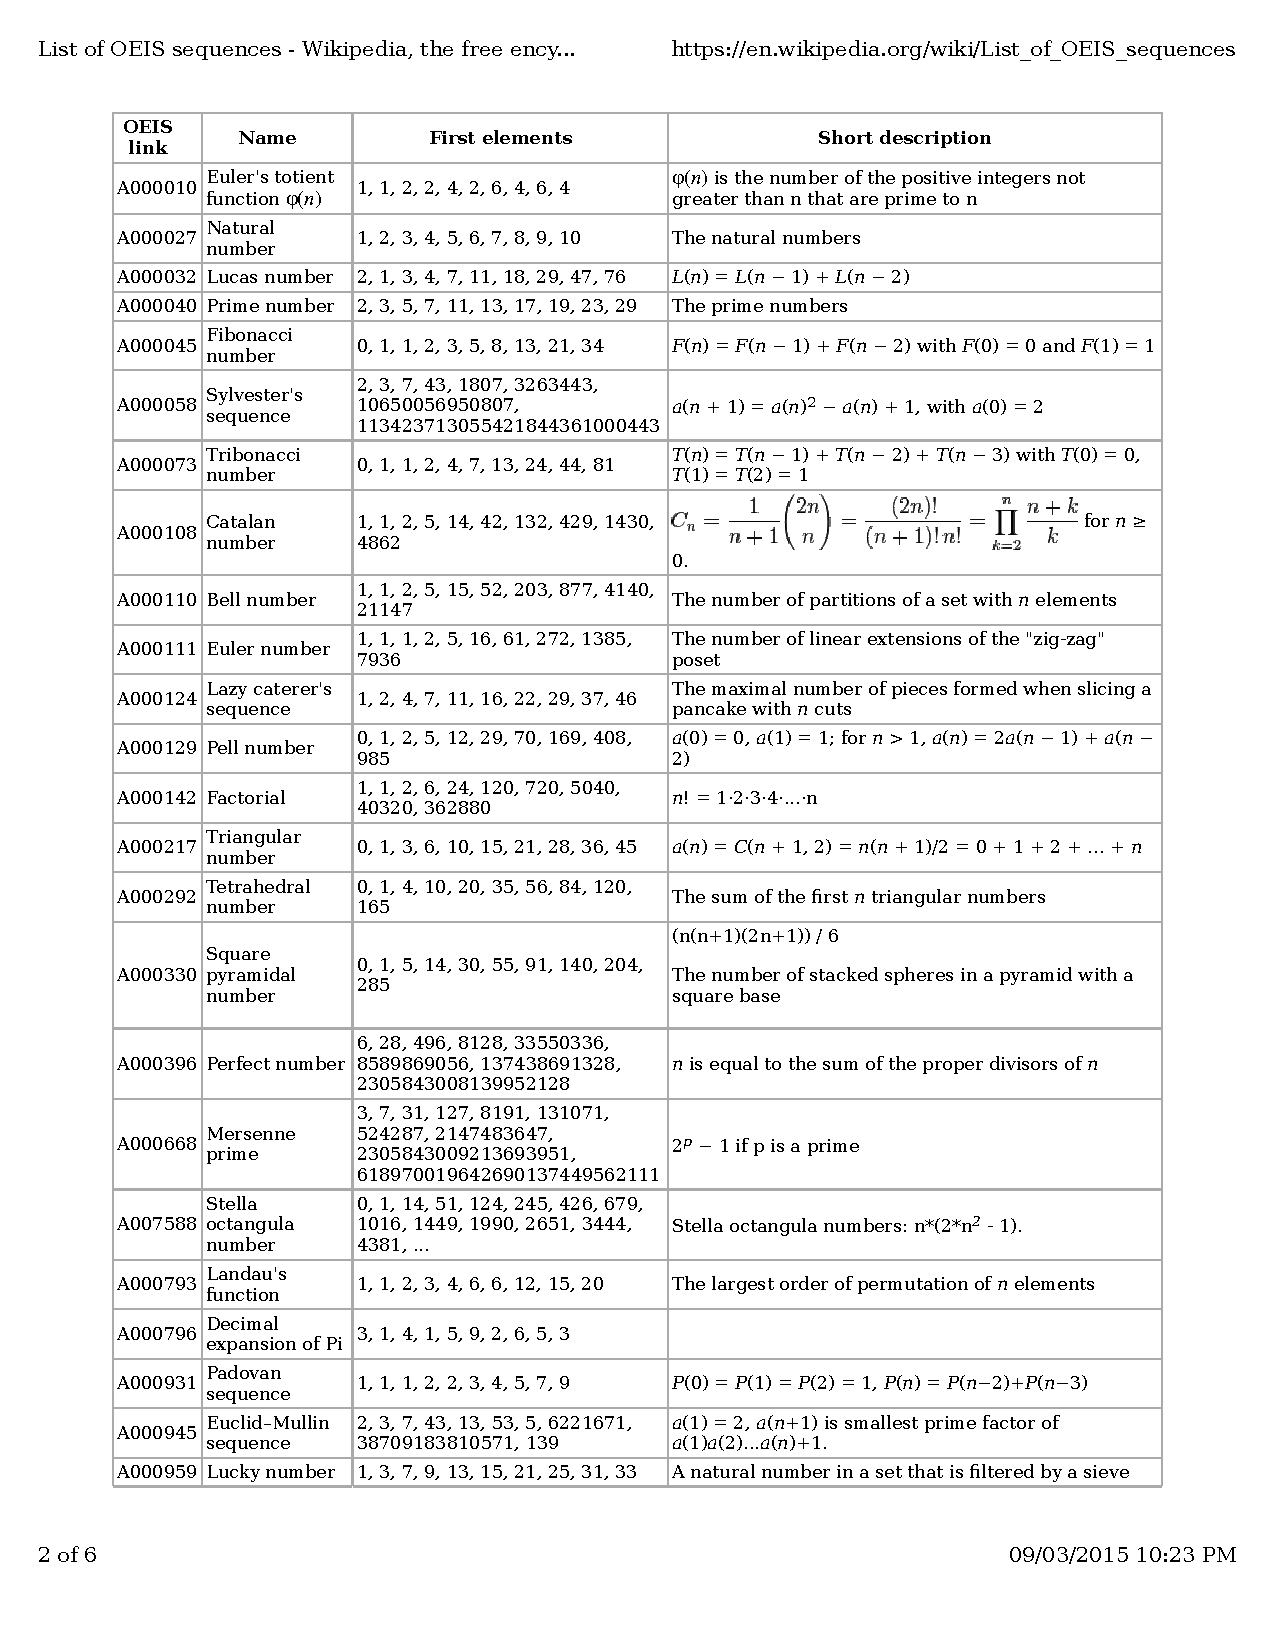
\includepdf[pages=-]{src/pdf-math/secuences.pdf}

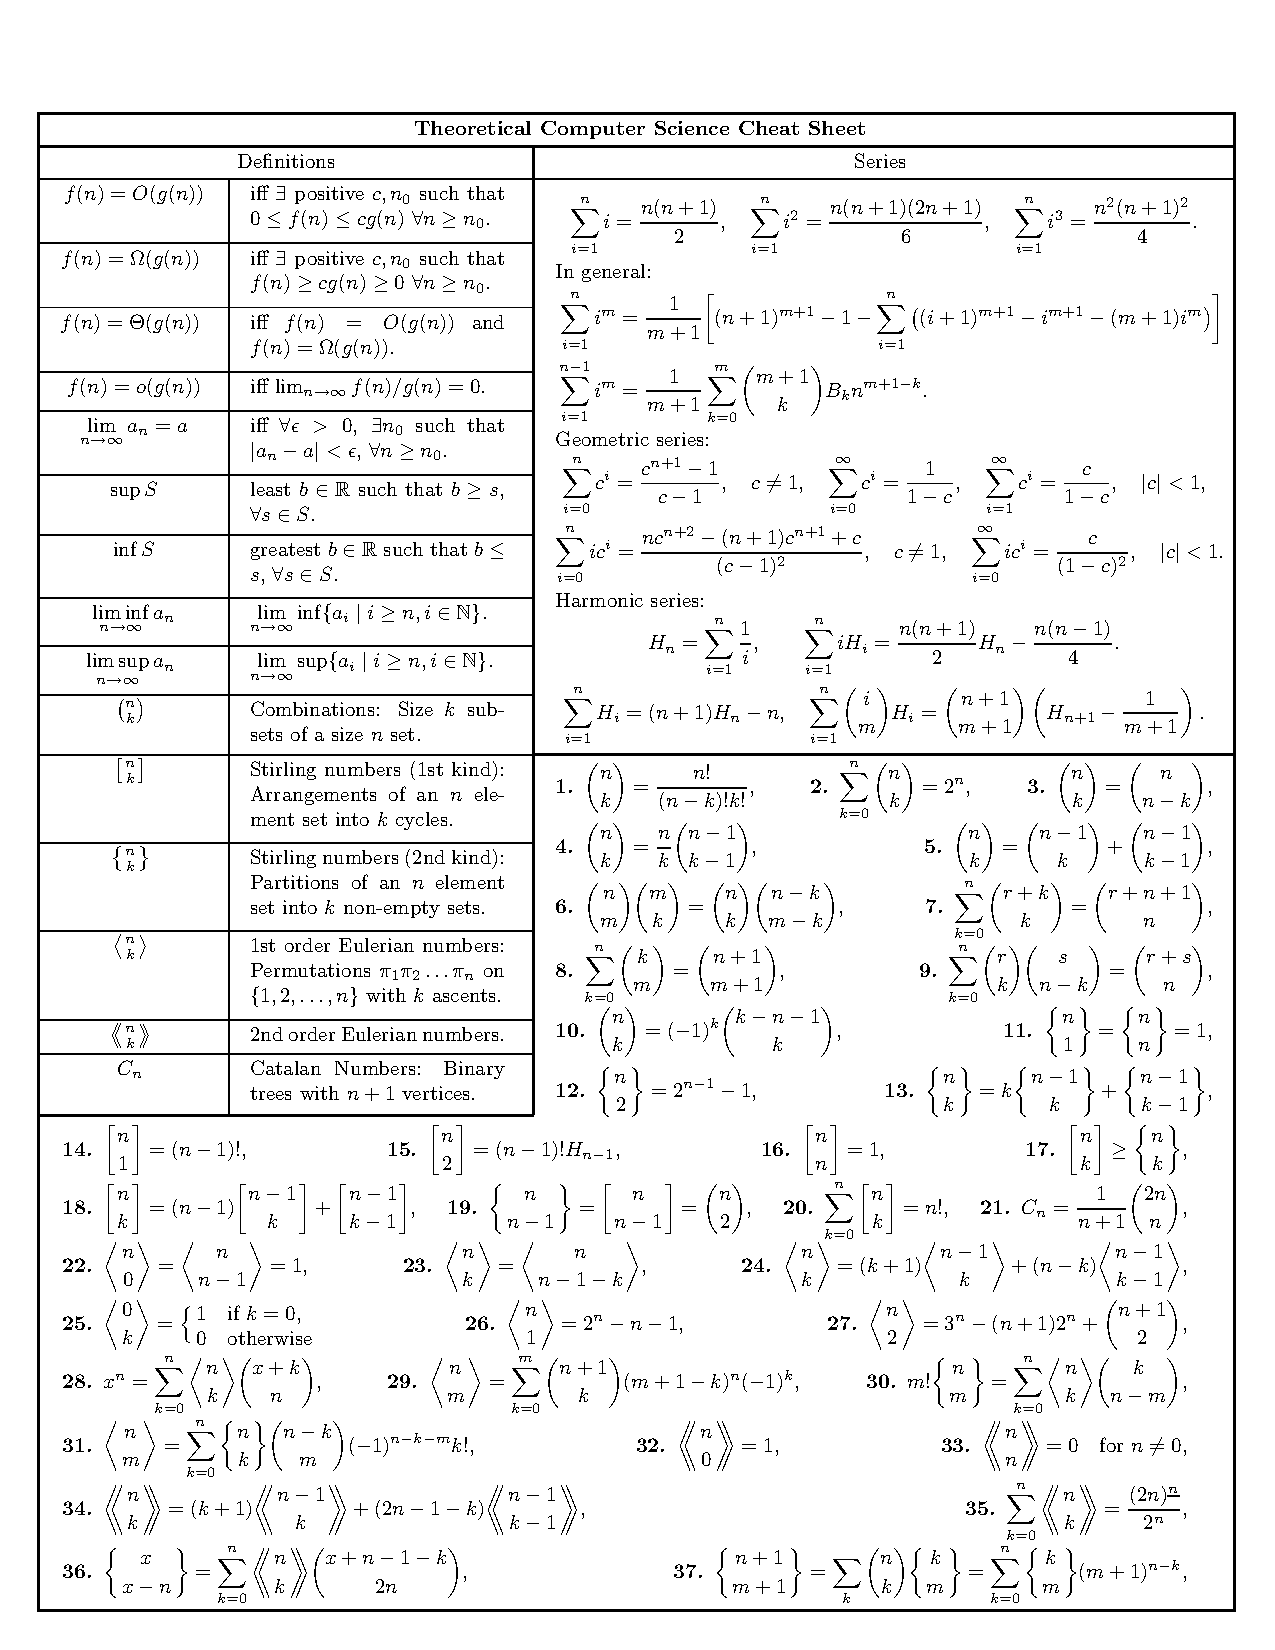
\includepdf[pages=-]{src/pdf-math/cheatsheet-math.pdf}
\end{document}